
\input{header}
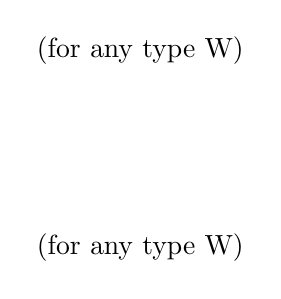
\begin{tikzpicture}[scale=1, transform shape]

\newnamedcomponent{0}{2.5}{GreeterImpl1}{GreeterImpl}
\newnamedcomponent{0}{0}{GreeterImpl2}{GreeterImpl}
\umlprovidedinterface[interface=GreeterImpl<W>, distance=3.2, padding=0.9cm]{GreeterImpl1}
\umlrequiredinterface[interface=W, distance=2.5, padding=0.9cm]{GreeterImpl1}
\node at (4.5,2.8) {(for any type W)};
\umlprovidedinterface[interface=std::function<std::unique\_ptr<GreeterImpl<W>{}>()>, distance=5.9, padding=0.9cm]{GreeterImpl2}
\umlrequiredinterface[interface=W, distance=2.5, padding=0.9cm]{GreeterImpl2}
\node at (4.5,0.3) {(for any type W)};

\end{tikzpicture}
\input{footer}
